%!TEX root = ../main.tex

\chapter{Results}\label{cha:results}

In this chapter, the implementation of a fingerprint function within the Axelrod-Python library will be examined.
This includes the addition of two strategy transformers, the Dual and JossAnn as defined in \ref{}. %TODO
Then several results will be presented where analytical fingerprints are compared with analytical ones.
A discussion that compares different fingerprints of strategies within Axelrod-Python will also be given.

\section{The Dual}
The dual of a strategy is defined such that when when the original strategy and the dual are presented with identical histories they will return opposite actions.
This relies on knowledge of how the original strategy would have behaved in a given situation, would be impractical to infer from the source code, however, the required behaviour can be achieved by having the original strategy as an attribute of the dual.
Whenever the dual has to submit a move, it can first get the original strategy to suggest what move should it would have made, and then flip that action.

\IncMargin{1.2em}
\begin{algorithm}[H]
 \KwData{A strategy}
 \KwResult{The d of the strategy}{}
  \If{First Turn}{
   create copy of original strategy\;}
  simulate original strategy\;
  update original strategy's history/internal state\;
  \Return{Flip of original strategy's move}
 \caption{The Dual of a Strategy}
\end{algorithm}\DecMargin{1.5em}

\section{Comparison of Analytical and Numerical Plots}

In figure \ref{fig:ashlock-fingerprints}, several analytical fingerprints from previous literature are shown \cite{Ashlock2004}.
Colourings and shadings are used to make certain features stand out, and an attempt to replicate this behaviour was implemented in Axelrod-Python.
The popular plotting library matplotlib has many options for different colour maps which are demonstrated in Appendix . %TODO

\begin{figure}[hbtp!]
    \begin{center}
        \includegraphics[width = 0.6\textwidth]{../img/MultipleFingerprintsAshlock}
    \end{center}
    \caption{Shaded plots of the fingerprint functions for the strategies TitForTat, Psycho, AllD and AllC, in reading order.}
    \label{fig:ashlock-fingerprints}
\end{figure}

Using the analytical fingerprints from previous literature, and the fingerprint formulae provided alongside them, the most appropriate colour map was chosen.
The colour map Seismic was selected due to its divergent properties (although all colour maps are available within the library).
With divergent colour maps, all extreme values (high or low) are coloured, whilst mid range values are left white.
This highlights areas of interest, and in Figure \ref{fig:WSLS-ashlock-comparison} it can be seen that this matches previous work very well.

\begin{figure}[hbtp!]
\centering
\subfloat[WSLS fingerprint from previous literature]{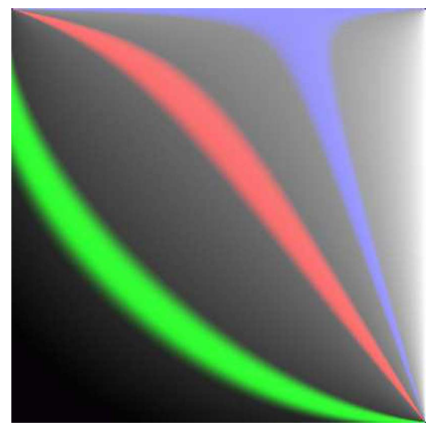
\includegraphics[width = 0.4\textwidth]{../img/WSLS-Ashlock}}
\subfloat[Analytical WSLS fingerprint demonstrating Seismic colouring]{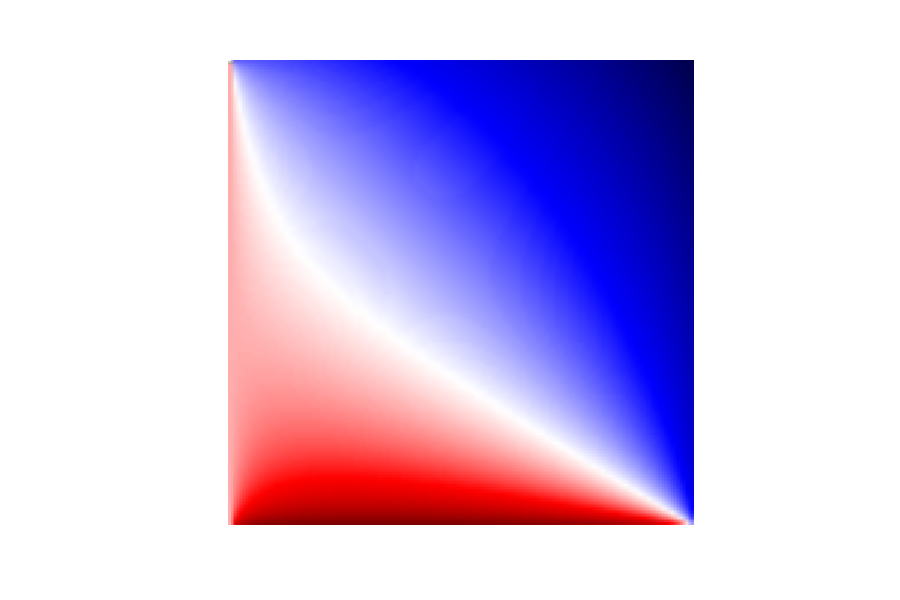
\includegraphics[width = 0.7\textwidth]{../img/WSLS-Analytical}}
\caption{A comparison of a fingerprint plot from previous literature to asses the suitability of the Seismic colour map}
\label{fig:WSLS-ashlock-comparison}
\end{figure}

With the knowledge that the choice of colourmap is appropriate, a comparison can now be made between analytical fingerprints and numerical ones obtained via the Axelrod-Python library.
Table gives the fingerprint functions of several well known strategies that will then be used to validate the numerical versions.

\begin{table}[htbp]
\centering
\renewcommand{\arraystretch}{2}
\setlength{\tabcolsep}{12pt}
\begin{tabular}{l l}
\toprule
Strategy & Analytical Fingerprint Function\\
\midrule
TitForTat &  $\displaystyle \frac{y^2 + 5xy + 3x^2}{(x + y)^2} $\\
Psycho (Anti TitForTat& $\displaystyle \frac{4(y-1)(x-1) + 5(y-1)^2}{2(y-1)(x-1) + (x-1)^2 + (y-1)^2} $ \\
WinStayLoseShit (Pavlov) & $\displaystyle \frac{(3x+y)(x-1) + 5y(y-1)}{(x+2y)(x-1) + y(y-1)} $\\
AllC (Cooperator) & $\displaystyle 3 - 3y $ \\
AllD (Defector) & $\displaystyle 4x + 1 $\\
\bottomrule
\end{tabular}
\label{tab:fingerprint-functions}
\caption{A selection of exact fingerprint functions for well known strategies. The probe used is TitForTat.}
\end{table}
